\documentclass[11pt]{IEEEtran}

\usepackage{graphicx}			% Inclusão de gráficos
\usepackage[justification=centering]{caption} % center caption

% \usepackage{microtype} 			% para melhorias de justificação
% \usepackage[T1]{fontenc}		% Selecao de codigos de fonte.
% \usepackage{float}

\usepackage{cite}
\usepackage{hyperref}
\hypersetup{
    colorlinks=true,
    linkcolor=blue,
    filecolor=blue,      
    urlcolor=blue,
}

\urlstyle{same}

% Your packages go here
\usepackage[utf8]{inputenc}
\usepackage{listings}
\usepackage{xcolor}   % for \textcolor
\lstset{
	basicstyle=\ttfamily,
	columns=fullflexible,
	frame=single,
	breaklines=true,
	postbreak=\mbox{\textcolor{red}{$\hookrightarrow$}\space},
}

\markboth{MO445 - Image Analysis}{}

\begin{document}
\title{Task 1}
\author{
Octávio Telles Teichner, 230148, o230148@dac.unicamp.br
}
\maketitle
    
\begin{abstract}

In order to extract numbers from the plates of images of cars, this first task aims to apply basic image processing methods such that the numbers are enhanced and every other element is minimized. 

The steps taken in order to achieve such results include pseudo-colorizing the original images (which were in gray-scale), changing their color spaces, applying batch normalization to limit the range of each pixel's intensity, creating random kernel banks, applying convolutions with said kernel banks and, at last, applying ReLU (Rectified Linear Unit).
\end{abstract}

\section{Introduction}

The optical signals that compose an image can be represented as single, quantified elements known as pixels \cite{foley1982fundamentals}. As such, each pixel, with its own set of coordinates and color values, represents the smallest element of an image.

The most common quantities attributed to a pixel are related to its spatial location and to its intensity. That is, where it resides within the image, which in 2D images is a set of (\textit{x, y}) coordinates and how bright (or how colorful) it is, respectively.

This first task aims to perform simple operations regarding these common quantities in order to extract useful information from images. More specifically, it aims to enhance the plate numbers of cars by using different color maps, normalizing, convolving and using activation functions.





Before moving on, a brief description of such operations is due. In short, 
applying different color maps to the pixels, which basically turns a gray-scale image into a pseudo-colorized image.

\section{Discussion}

Given a data set composed of several gray-scale images, each with one car and one plate, the first step was to organize the data-set in a way that the data contained basically just the plates and nothing else.

To achieve this, several functions are defined in the \textbf{main.py} file, which is at the root of the repository found here
\url{https://github.com/otthtml/mo445-task1}.

Since an image can be read simply by calling OpenCV's very useful function \textit{imread}, it was only necessary to apply a HSV color map to the image, which was read and converted into a NumPy array (another very useful library). The function can be found below.

\begin{lstlisting}[language=Python]
def turnIntoYCbCr(image: np.ndarray):

    image = cv2.applyColorMap(image, cv2.COLORMAP_HSV)
    image = cv2.cvtColor(image, cv2.COLOR_HSV2RGB)
    image = cv2.cvtColor(image, cv2.COLOR_RGB2YCrCb)

    return image.astype(np.float32)
\end{lstlisting}

As the name of the functions make it pretty self-explanatory, this excerpt of code converts the image into the YCbCr color space, where Y is the \textit{luminance} component and Cb and Cr are the blue-difference and red-difference \textit{chroma} components, respectively.

In the last line, this function also converts each element of the image (or NumPy array), from an integer to a floating point, which is crucial to future operations (such as the normalization).

The \textit{turnIntoYCbCr} function is used inside the \textit{createSubImage} function, which effectively tried to extract just the plate from the image given a binary mask which basically points where the plate is. 

The \textit{createSubImage} function takes two NumPy arrays as parameters, one representing the image, the other representing the mask of the image, both with the same dimensions (but different color spaces). The function then ``slides'' a window of predetermined size (defined by the ``WIDTH'' and ``HEIGHT'' constants) over the mask and calculates the ratio between the white pixels (which are the pixels that belong to the plate) and the total amount of pixels in the window.

At the end of each iteration, if the current window has a better ratio than the last window, then it'll be selected as the best candidate to contain the plate. This was prefered over the original requirement of the task, which was to implement a threshold, where the first ratio that exceeded such threshold would be immediately returned.

By the end of the function, there's also an exception clause, which is required to handle cases where the sliding window exceeds the mask's dimensions (an index error, basically). After all iterations, the best candidate is submitted through the \textit{turnIntoYCbCr} function and returned.

With a more ``precise'' image in hands (again stored as a NumPy array), we apply the \textit{batchNormalization} function to it, which basically reduces the range of each pixel (originally 0-255). As one can see in the function below, each channel is normalized individually.

\begin{lstlisting}[language=Python]
def batchNormalization(image: np.ndarray):

    for j in range(image.shape[2]):
        s = image[:, :, j].shape[0] * image[:, :, j].shape[1]
        mean = np.sum(image[:, :, j]) / s
        deviation = sqrt(( np.sum( (image[:, :, j] - mean)**2 ) ) / (s - 1))
        image[:, :, j] = (image[:, :, j] - mean)/deviation

    return image
\end{lstlisting}

All that's left is to generate our kernel bank, with kernels that have random coefficients, and apply one convolution for each kernel generated. All of this can be achieved by instantiating the class \textit{KernelBank} - which takes two arguments, the shape of each filter (3 in this case) and the size of the filter bank (which is defined as an environment variable in this case) - and calling its \textit{convolve} function, which applies a convolution for each kernel generated and returns an array of images.

As with every convolution, the borders of the image are often subject of discussion. There are several methods to handle the ``unreachable'' pixels that extend beyond the image, but are still required by the kernel. For example, one can simply add some zero-padding to the original image, which basically nullifies the elements of the kernel that extend beyond the original image, which is what the parameter ``method'' did when set to ``constant''.

Each image generated can then be easily displayed and saved by looping through the results array (which contains the convolved images) and using the very useful Matplotlib library. For comparison's sake, a vertical Sobel kernel was also convolved with the same image.

\begin{lstlisting}[language=Python]
for i in range(len(results)):
    plt.figure()
    plt.imshow(results[i])
    plt.savefig('./output/patches/'+ name + '_' + str(i) +'.png')
    plt.close()
\end{lstlisting}


\section{Results}

Each of the five steps described in the project \cite{task1} produces at least one image, which makes it easier to gradually show the results. The intermediary results are only present in this report and are not included as the output of the source code.

First, as the data set of images is read, each plate appears to be successfully isolated, as shown in the figure \ref{1}, and converted to the YCrCb color space (after being pseudo-colorized to a HSV color map), as shown in the figure \ref{2}. The result isn't very satisfying, as applying a HSV color map to the image actually seems to make it harder to recognize the plate numbers.

\begin{figure}[h!]
    \centering
    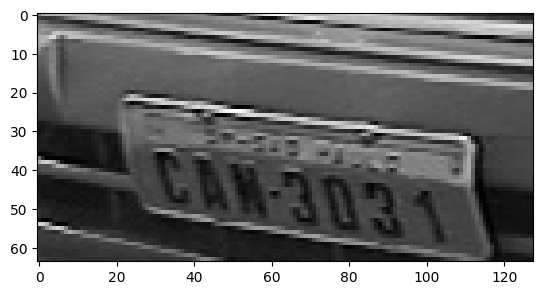
\includegraphics[width=0.4\textwidth]{article1/1.png}
    \caption{Plate extraction}
    \label{1}
\end{figure}

\begin{figure}[h!]
    \centering
    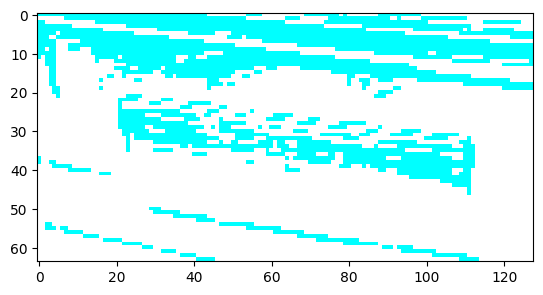
\includegraphics[width=0.4\textwidth]{article1/2.png}
    \caption{Pseudo-colorization}
    \label{2}
\end{figure}

However, after applying the \textit{batchNormalization} function to the same unrecognizable image, the range of each pixel's intensity is reduced to (-1, 1), approximately, which greatly improved the distinction of the plate numbers (somehow), as can be noticed in figure \ref{3}.

\begin{figure}[h!]
    \centering
    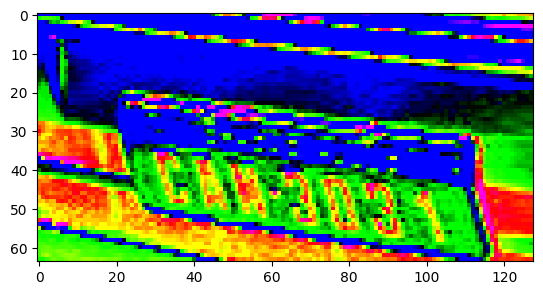
\includegraphics[width=0.4\textwidth]{article1/3.png}
    \caption{Batch normalization}
    \label{3}
\end{figure}

However, after applying the \textit{batchNormalization} function to the same unrecognizable image, the range of each pixel's intensity is reduced to (-1, 1), approximately, which greatly improved the distinction of the plate numbers (somehow), as can be noticed in figure \ref{3}.

However, after applying the \textit{batchNormalization} function to the same unrecognizable image, the range of each pixel's intensity is reduced to (-1, 1), approximately, which greatly improved the distinction of the plate numbers (somehow), as can be noticed in figure \ref{3}.

Inside the \textit{convolve} function, there is a commented section which applies a convolution using only one channel of the kernel and then rebinds the three channels together into one image, as shown in the piece of code below.

\begin{lstlisting}[language=Python]
result0 = signal.convolve2d(image[:,:,0], self.kernels[i][:,:,0], mode='same')
result1 = signal.convolve2d(image[:,:,1], self.kernels[i][:,:,0], mode='same')
result2 = signal.convolve2d(image[:,:,2], self.kernels[i][:,:,0], mode='same')
result = np.zeros( (WIDTH, HEIGHT, 3) )
result[:,:,0] = result0
result[:,:,1] = result1
result[:,:,2] = result2
\end{lstlisting}

Since this approach used only one channel of the kernel (equivalent to a kernel of norm equal to one) the results are less random between the images of the same kernel bank, even though it's less efficient and more verbose than the simple \textit{ndimage.convolve} method, which is also present in the source code and is not commented.

The last step, the activation function is simply applied inside the \textit{convolve} function, with the excerpt of code described below, which basically nullifies any pixels with intensity lower than 0, effectively reducing the range of values even more than with just the batch normalization.

\begin{lstlisting}[language=Python]
self.results.append( np.maximum(result, 0) )
\end{lstlisting}

The difference between this custom convolution with a random kernel and the convolution with the famous vertical Sobel kernel can be expressed by its results. In figure \ref{4}, we have the image generated by our custom convolution which also applies the activation function.

\begin{figure}[h!]
    \centering
    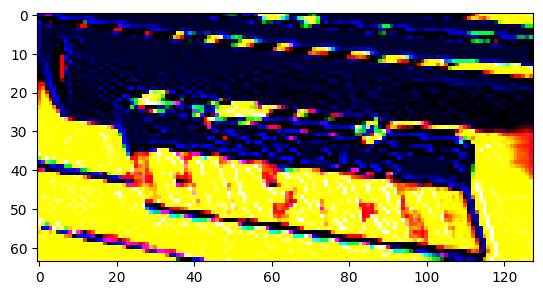
\includegraphics[width=0.4\textwidth]{article1/4.png}
    \caption{Custom convolution}
    \label{4}
\end{figure}

In figure \ref{5}, we have the image generated just by convolving the vertical Sobel kernel, which aims to enhance vertical edges. As one can notice, both results fail to enhance the plate number, but the Sobel filter manages to ``delete'' some part of the background.

\begin{figure}[h!]
    \centering
    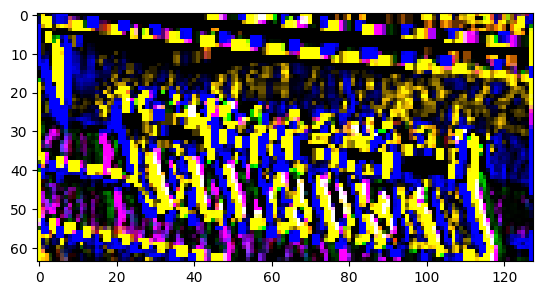
\includegraphics[width=0.4\textwidth]{article1/5.png}
    \caption{Custom convolution}
    \label{5}
\end{figure}

\section{Conclusions}

This entire project proved to be a challenge. Implementing some functions, creating our filters, tackling common image processing challenges such as pseudo-colorization, normalization and multi-band convolutions, all of this has proportioned a great amount of experience.

The results proved to be somewhat underwhelming, mostly due to the unnecessary color map that was applied to every image. The plate number, which was already pretty distinguishable in figure \ref{1}, turned into a colorful painting, where no combination of operations (and kernels) succeeded in enhancing its characters, as seen in figure \ref{4}.


\bibliographystyle{plain}
\bibliography{document}


\end{document}
